% MATLAB source: verification/crack_path/main_tip_core_mesh_level_comparison.m
% H2 is a mesh-family visualization only; H1 and H0 satisfy the established
% native COD sampling gate. Panel letters are supplied by LaTeX.
\begin{figure}[tbp]
  \centering
  \begin{subfigure}[t]{0.315\linewidth}
    \centering
    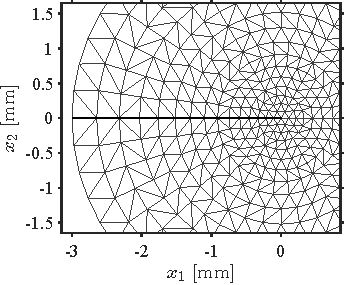
\includegraphics[width=\linewidth]{figures/mesh_levels/tip_mesh_H2.pdf}
    \caption{$4h_0$: $h_{\mathrm{tip}}=0.1080493$ mm.}
    \label{fig:mesh-level-H2}
  \end{subfigure}
  \hfill
  \begin{subfigure}[t]{0.315\linewidth}
    \centering
    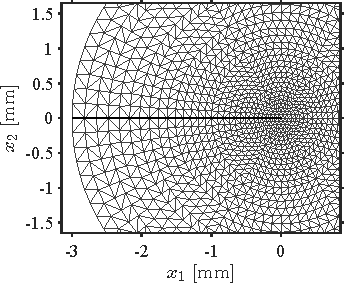
\includegraphics[width=\linewidth]{figures/mesh_levels/tip_mesh_H1.pdf}
    \caption{$2h_0$: $h_{\mathrm{tip}}=0.0540247$ mm.}
    \label{fig:mesh-level-H1}
  \end{subfigure}
  \hfill
  \begin{subfigure}[t]{0.315\linewidth}
    \centering
    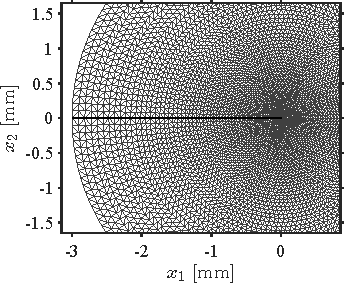
\includegraphics[width=\linewidth]{figures/mesh_levels/tip_mesh_H0.pdf}
    \caption{$h_0$: $h_{\mathrm{tip}}=0.0270123$ mm.}
    \label{fig:mesh-level-H0}
  \end{subfigure}

  \caption{Structured near-tip mesh hierarchy at fixed core radius
  $r_c=3$ mm, where $h_0=0.0270123$ mm is the production tip size.
  The panels use identical local coordinates and spatial limits. The
  $2h_0$ and $h_0$ meshes satisfy the established native COD-sampling
  requirement. The $4h_0$ mesh is included only to illustrate the geometric
  resolution hierarchy: its four COD windows contain 10, 15, 12, and
  9 native points, so it is not admitted as a physically qualified mesh.}
  \label{fig:mesh-levels}
\end{figure}
